% This is based on the LLNCS.DEM the demonstration file of
% the LaTeX macro package from Springer-Verlag
% for Lecture Notes in Computer Science,
% version 2.4 for LaTeX2e as of 16. April 2010
%
% See http://www.springer.com/computer/lncs/lncs+authors?SGWID=0-40209-0-0-0
% for the full guidelines.
%

\documentclass{llncs}
\usepackage{graphicx}
\usepackage[english]{babel}
\usepackage{cleveref}
\usepackage{hyperref}

\newcommand{\quotes}[1]{``#1''}

\begin{document}

\title{PARSIAN 2018\\Extended Team Description Paper}
%
\titlerunning{PARSIAN 2018 ETDP}  % abbreviated title (for running head)
%                                     also used for the TOC unless
%                                     \toctitle is used
%
\author{Mohammad Mahdi Rahimi \and Mohammad Mahdi Shirazi \and \\
Mohammad Amin Najaf Gholyan \and Fateme Hashemi Chaleshtori\and Nadia Moradi \and Kian Behzad \and Seyed Hamidreza Roodabeh \and Ali Gavahi \and Fateme Farokhi Moghadam  \and Seyed Ali Ghazi Asgar \and Yasamin Alizadeh Gharib\and Mahshid Memarian \and Amir Hadi Tavakoli \and Mohammad Azam Khosravi}
%
\authorrunning{Mohammad Mahdi Rahimi et al.} % abbreviated author list (for running head)
%
%%%% list of authors for the TOC (use if author list has to be modified)
\tocauthor{Mohammad Mahdi Rahimi, Mohammad Mahdi Shirazi,Mohammad Amin Najaf Gholian, Fateme Hashemi , Nadia Moradi, Fateme Moghadam, Kian Behzad, Hamidreza Roodabeh, Ali Gavahi, and Mohammad Azam Khosravi}
%
\institute{	
	Electrical Engineering Department\\
    Amirkabir Univ. Of Technology (Tehran Polytechnic) \\
    424 Hafez Ave. Tehran, Iran\\
	\email{
    	\{mmrahimi,mhmmdshirazi,hashemi96,nadiamoradi,kian.behzad,hr.roodabeh,\\aligavahi,fateme.fmoghadam,alizadeh\_yasi,m.a.khosravi\}@aut.ac.ir 
    }
	\texttt{http://www.parsianrobotics.aut.ac.ir}
}

\maketitle              % typeset the title of the contribution

\begin{abstract}
This paper presents Parsian's hardware elaboration, the software architecture and all improvements that have been made since last year, including useful innovations in hardware, e.g. new ball detection sensor, debugger module and robot's fault recovery. Noteworthy enhancements in software such as micro-service architecture by ROS, open loop motion correction, motion profiler and new obstacle avoidance strategy are described.


\keywords{microservice, ROS, motion control, fault recovery}

\end{abstract}
%
\section{Introduction}
%
Parsian Robocup Soccer team formed in 2005 by Electrical Engineering Department of Amirkabir University of Technology, and has been working on small size league since then. This team aims to design and build SSL robots, compatible with international RoboCup competition rules as an engineering project. This team has been qualified for twelve consequent years for RoboCup SSL, and participated in 2008 to 2017 RoboCup competitions. Parsian's most significant success is first place in RoboCup 2012 and RoboCup 2013 technical challenges and also fourth place in RoboCup 2012 and 2017.
%
\newpage

\subsection{Team members}
%
Mohammad Azam Khosravi: Control Theory, Supervisor \newline
Mohammad Mahdi Shirazi: Control, Firmware, Team Leader \newline
Mohammad Mahdi Rahimi: AI Software \newline
Mohammad Amin Najaf Gholian: Electronic, Mechanic \newline
Fateme Hashemi Chaleshtori: AI Software \newline
Nadia Moradi: AI Software \newline
Kian Behzad: AI Software \newline 
Seyed Hamidreza Roodabeh: AI Software \newline 
Ali Gavahi: AI Software \newline
Fateme Farokhi Moghadam: Electronic \newline
Seyed Ali Ghazi Asgar: Electronic \newline
Yasamin Alizadeh Gharib: Electronic \newline 
Mahshid Memarian: Mechanic \newline
Amir Hadi Tavakoli: AI Software
%
\section {Hardware}
%
\subsection{Mechanic}
\subsubsection{Motor and Gearbox.}
\label{subsubsec:MotorAndGearbox}
This year the gear ratio has been changed from 3.6:1 to 2.5:1, to increase the maximum velocity.
The major innovation is changing the angle of the wheels' cone, so that the robot's center of mass can be lowered and solenoids can be flattened as well.
In this concept, the chip's rocker shaft has been raised since it has a higher transient impulse power, and chip solenoid core collides to the center of percussion of chip shaft.
\subsubsection{Dribbler and Spin.}
\label{subsubsec:DribblerAndSpin}
At the back of the dribbler, a spring-damper system has been placed. According to the mass of the dribbler and the ball, it will be over-damped at high speeds (over 10m/s). Since the relative stiffness of the dribbler causes spin disruption and resonance in the movement of the ball, this is not the perfect solution. So the chosen damper, has the ability to be calibrated for different carpets.

\subsection{Electronic}
\label{subsec:Electronic}
\subsubsection{Kick Sensor.}
\label{subsubsec:KickSensor}
To detect the ball, infrared transmitter and infrared receiver sensors are embedded in both sides of the robot's dribbler.
    In the previous design, a typical IR photo-diode sensor has been used that was highly affected by ambient light. In the new design, a typical IR LED is used, along a TSOP1238 to receive the infrared signals.
    \newline
    Each member of TSOP12xx series is sensitive to different frequencies of IR spectrum; the xx shows the frequency that the sensor detects.
    For generating the IR signals at 38Khz, a 555 Timer IC is used in astable multi-vibrator mode. In this mode, it works as a free running oscillator and generates approximately 38 kHz square waves.
   
\subsubsection{Debug Mode.}
\label{subsubsec:DebugMode}
Last year essential data such as battery voltage, wireless data-lost ratio, motors’ fault and other failures has been sent to communication module. This year, besides that, debug part has been added to send robot's parameters including wheels’ speed, control variables, etc. for monitoring and analyzing.
\subsubsection{Fault Recovery.}
\label{subsubsec:FaultRecovery}
There’s two major methods in control for fault recovery procedure; (1) active fault recovery that means the control system is redesigned when a fault happens and (2) passive fault detection that means the control system is robust enough to tolerate probable fault.
\newline This year an active fault recovery has been implemented for motor-based faults. First of all if a motor connection has been unplugged or the motor has some failures like hall-sensor faults, the system’s kinematic is switched to an appropriate three-wheel kinematic; so the robot’s able to move, either to play the game with less efficiency or just to reach the legal substitution place in the field. 
\newline The second is the encoder fault that can happen because of different reasons like unplugged encoder socket or electrical failure. In this case the velocity measurement reference, is changed from encoder to the motor’s hall sensors.
\subsubsection{Optical Flow.}
\label{subsubsec:OpticalFlow}
PAN3401 is a CMOS process optical mouse sensor single chip with a PS/2 interface that serves as a non-mechanical motion estimation engine for implementing a computer mouse.
A CMOS image sensor sends each image to a digital signal processor (DSP) for analysis. The DSP operating speed is 18 MIPS. It can detect patterns in the images and compare them to the previous image. Based on the change in patterns over a sequence of images, the DSP determines how far the sensor has moved during a certain time. The movement measurement frequency is 100Hz.
This sensor will be used in future works as a local reference of linear velocities.

\section{Control}
%
 \subsubsection{Open-Loop Motion Correction.}
\label{subsubsec:OpenLoopMotionCorrection}
In order to achieve perfect motion control, a new learning-based method has been implemented which fixes open-loop motion errors.
In polar coordinates, the robots' movement is expressed as direction angle ($\theta$), velocity (V) and angular velocity ($\omega$). In this method, two offsets have been added to $\theta$ and $\Omega$; linear velocity is accurate enough and remains without offset.
\newline
At first, a PSO method was implemented with a complicated cost function to optimize multiple variables simultaneously; but after reviewing the results, it was realized that these two parameters ($\theta$ and $\omega$) are almost independent and a simple method can be employed separately, for each parameter.
\newline
One efficient method that can be utilized to optimize a parameter, is \textit{Error Back Propagation}. It's mainly used in finding weights of neural networks. The result of this method was satisfying; one instant is depicted in Fig. \ref{fig:control1}
\begin{figure}
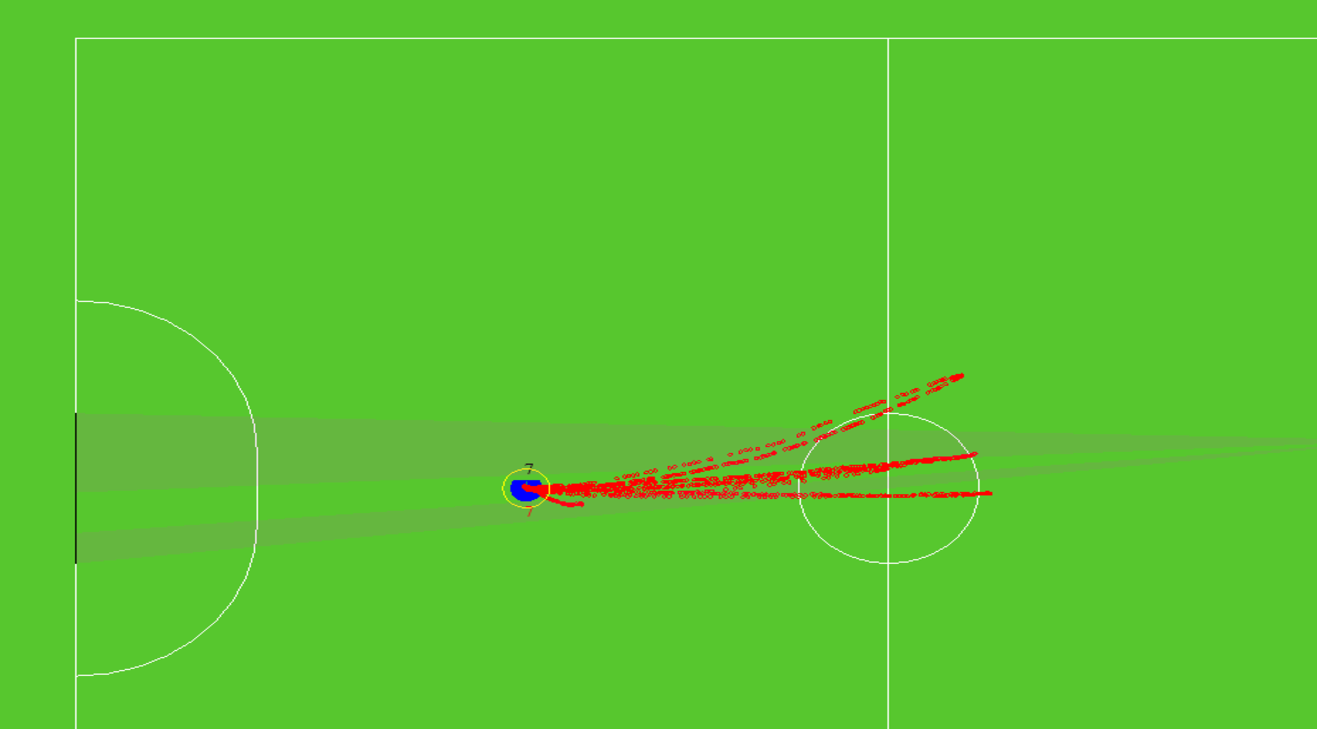
\includegraphics[width=\textwidth]{img/f1}
\caption{Open-loop motion learning}
\label{fig:control1}
\end{figure}

\subsubsection{Angle-base Deceleration.}
\label{subsubsec:AngleBaseDeceleration}
The robot’s maximum deceleration depends on the movement angle. Previously a constant deceleration had been used for all angles, but this year it was extended to three different decelerations, one for each of the forward, backward and normal angles. Desired deceleration for each angle will be calculated by a weighted average, depending on movement angle (Fig. \ref{fig:control2} and  \ref{fig:control3}).
\begin{figure}
%\centering
%\begin{minipage}{.2\textwidth}
\centering
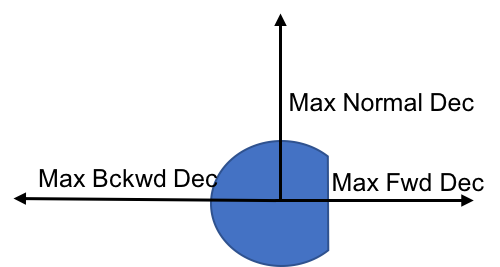
\includegraphics[width=.5\linewidth]{img/f2}
\caption{Deceleration in different angles}
\label{fig:control2}
%\end{minipage}
\centering
%\begin{minipage}{.72\textwidth}
\centering
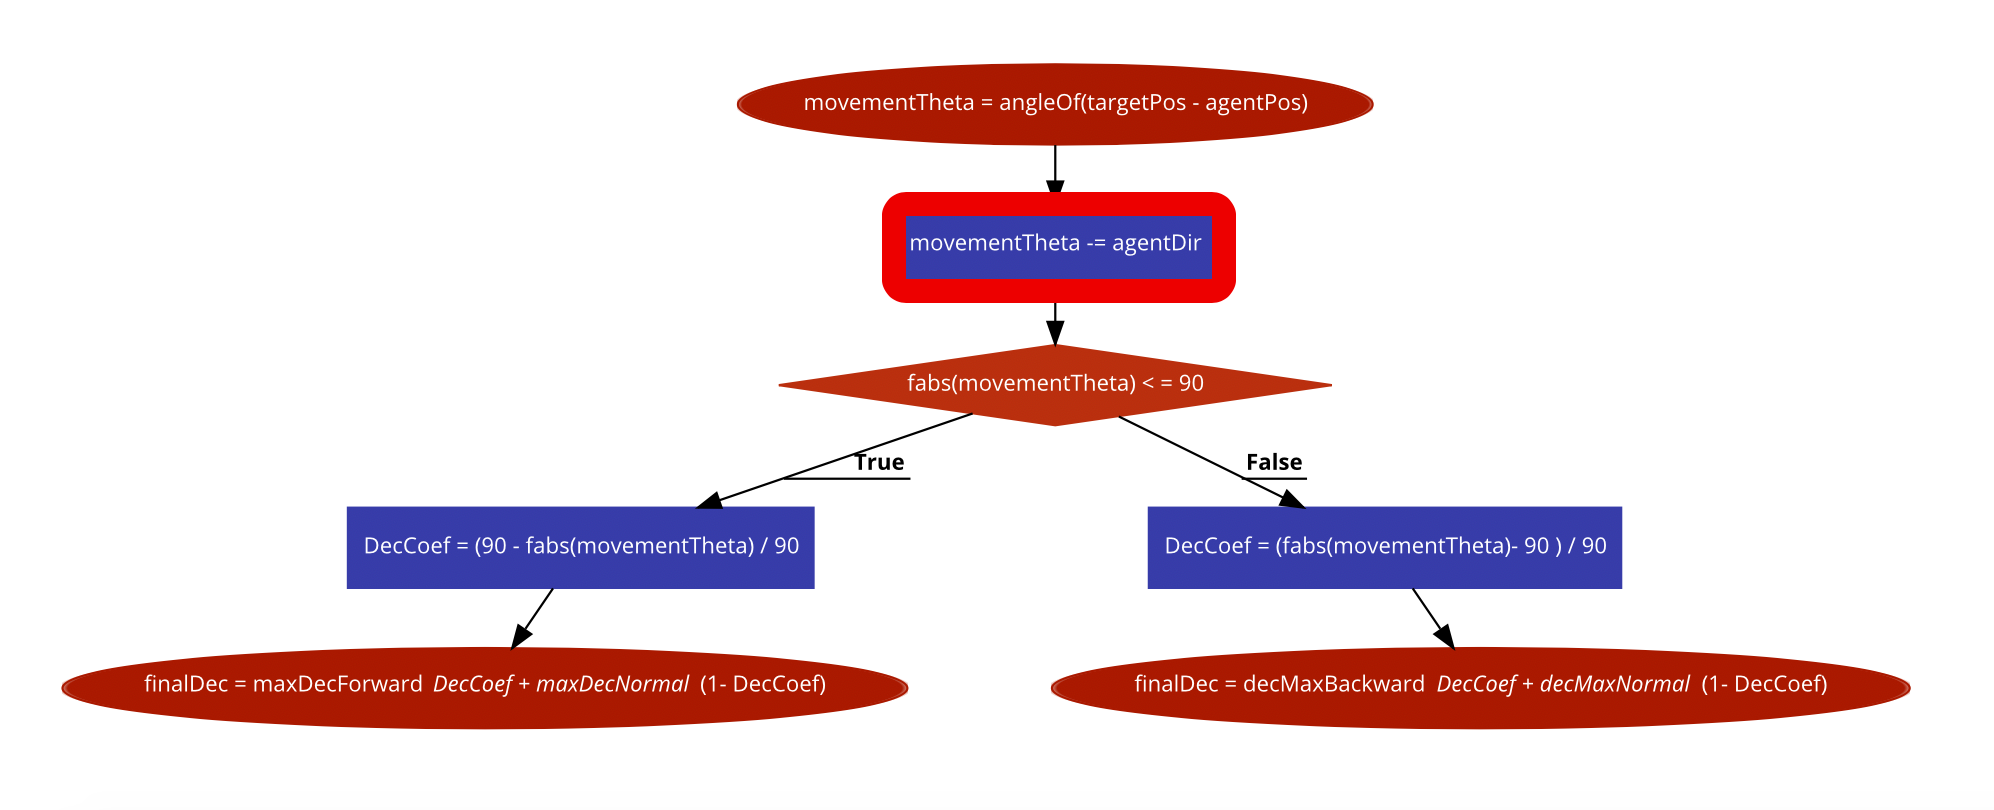
\includegraphics[width=\linewidth]{img/f3}
\caption{Flow-chart of calculating desired deceleration}
\label{fig:control3}
%\end{minipage}
\end{figure}

\subsubsection{Motion Profiler.}
\label{subsubsec:MotionProfiler}
Motion profiler is a module which moves a robot in different distances, angles, and directions. Then it records vision data, robot’s motion data and dispatched commands, also extracts useful information from these raw data (Fig. \ref{fig:motion1} and \ref{fig:motion2}).
\begin{enumerate}  
\item Robot velocity-time table of each motion
\item Remaining distance-time table of each motion
\item Command velocity-time table of each motion
\end{enumerate}
Then it calculates some useful information including:
\begin{enumerate}  
\item Total delay by calculating time shift between speed and command 
\item Time needed for a robot to move from one point to another, with four-dimensional regression on the raw data
\end{enumerate}

\begin{figure}
\centering
\begin{minipage}{0.45\textwidth}
\centering
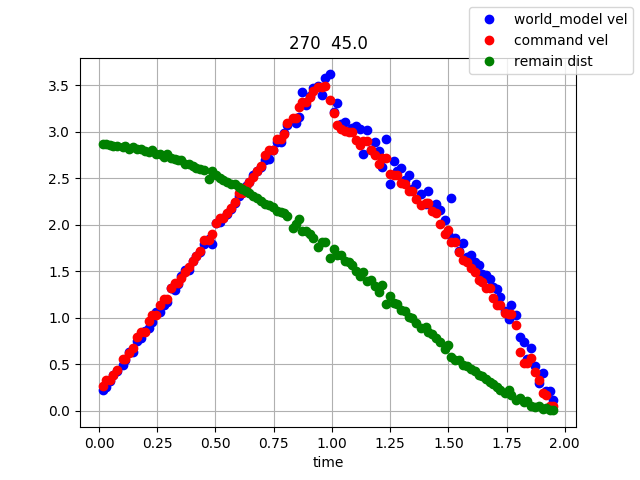
\includegraphics[width=\linewidth]{img/motion1}
\caption{Raw data which is collected for short path}
\label{fig:motion1}
\end{minipage}
\centering
\begin{minipage}{0.45\textwidth}
\centering
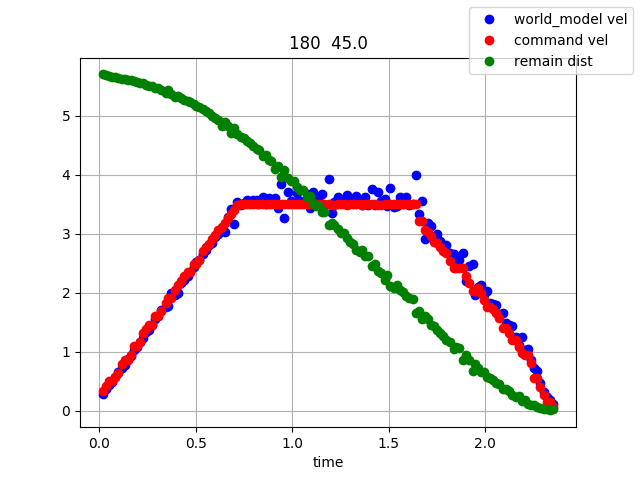
\includegraphics[width=\linewidth]{img/motion2}
\caption{Raw data which is collected for long path}
\label{fig:motion2}
\end{minipage}
\end{figure}

\newpage
\subsubsection{Obstacle Avoidance.}
\label{subsubsec:ObstacleAvoidance}
Parsian has been using \textit{ERRT} algorithm for years that is mostly used in real-time approaches. In order to decrease the number of collisions and also minimize the travel time, a new approach for obstacle avoidance has been developed. This method does not intend to change \textit{ERRT} implementation or propose a new way to avoid obstacles; it’s rather about how to define the obstacles space.
This method is based on opponent robots’ capabilities:
\begin{enumerate}  
\item Maximum Deceleration
\item Maximum Velocity
\item Agility Factor
\footnote{Agility Factor represents by how many degrees, the movement direction of a robot can change, during a specified time in its maximum velocity.}
\item Current Velocity 
\end{enumerate}
A probability area can be chosen for a certain upcoming time interval.
    If the probability area for opponent robots and future position of our robot overlaps, then the obstacle avoidance try to avoid that common space. (Fig. \ref{fig:obs1})

\begin{figure}
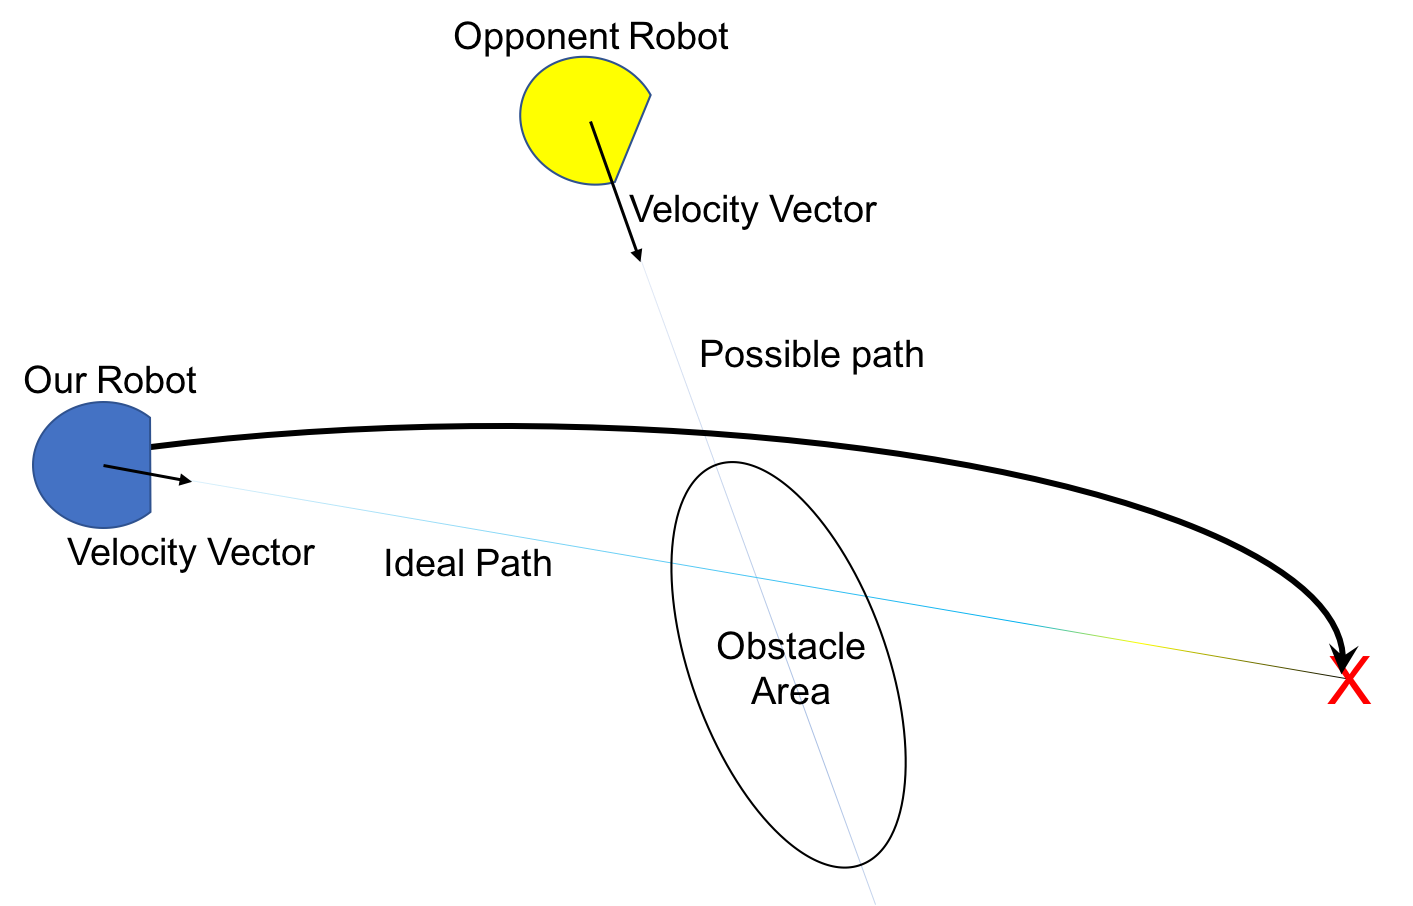
\includegraphics[width=\textwidth]{img/obs}
\caption{Generated path, considering overlap area}
\label{fig:obs1}
\end{figure}


%
\newpage
\section{Software}

\subsection{Microservice}
\label{subsec:Microservice}
Parsian Software has been splitted into different components and the monolithic based architecture has been altered to distributed. The new architecture has a lot of  benefits such as:
\begin{itemize}
  \item \textbf{Agility}: New features and products can be added more quickly.
  \item \textbf{Independent Deployment}: The components are easy to understand and modify; this can help a new team member become productive quickly.
	\item \textbf{Polyglotism}: Team has freedom to choose technology and programming language that is best suited for a particular functionality.
	\item \textbf{Better Fault Isolation}: If one component fails, there's a less chance to impact other ones, and they will continue to work.
	\item \textbf{Testability}: Test surface is smaller than that of monolithic applications thus it’s easier to be tested.
	\item \textbf{Easier Analysis}: The transferred messages leads to analyze the data in a more convenient way.
\end{itemize}

\subsection{ROS}
\label{subsec:ROS}
Robot Operating System (\textit{ROS}) is a collection of software frameworks for robot software development. ROS provides services designed for heterogeneous computer clusters such as hardware abstraction, low-level device control, implementation of commonly used functionality, message-passing between processes, and package management. Running sets of ROS-based processes are represented in a graph architecture, where processing takes place in nodes. Despite the importance of reactivity and low latency in robot control, ROS itself, is not a real-time OS (\textit{RTOS}), though it is possible to integrate ROS with real-time code.
There are three types of software In ROS ecosystem:
\begin{enumerate} 
	\item Language and platform-independent tools
	\item ROS client library such as roscpp, rospy, rosjava, etc.
	\item Packages containing application-related code by using ROS client libraries
\end{enumerate}

In Parsian project the control and AI nodes are written in C++ using roscpp. GUI, test nodes and tools like profilers are implemented with python scripts (rospy).

\subsection{Architecture}
\label{subsec:Architecture}
\subsubsection{Package.}
\label{subsubsec:Package}
Parsian Stack (ROS repository), packages and their dependencies graph, are shown in  Fig. \ref{fig:AI1}.

Packages are the first-level directory that separate source codes; so to implement a package for the first time, debug, upgrade or even re-factor it, only that particular package and its dependencies need to be changed.

\begin{figure}
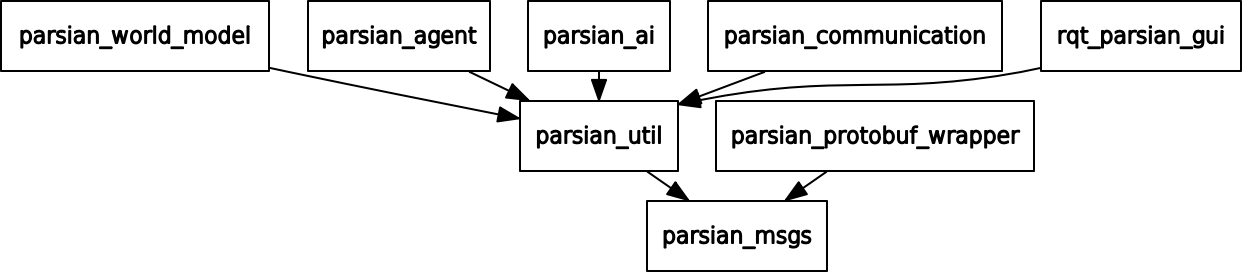
\includegraphics[width=\textwidth]{img/ai1}
\caption{Parsian packages graph}
\label{fig:AI1}
\end{figure}

First-level dependencies of Parsian packages to ROS packages are shown in Fig. \ref{fig:AI2}:
\begin{figure}
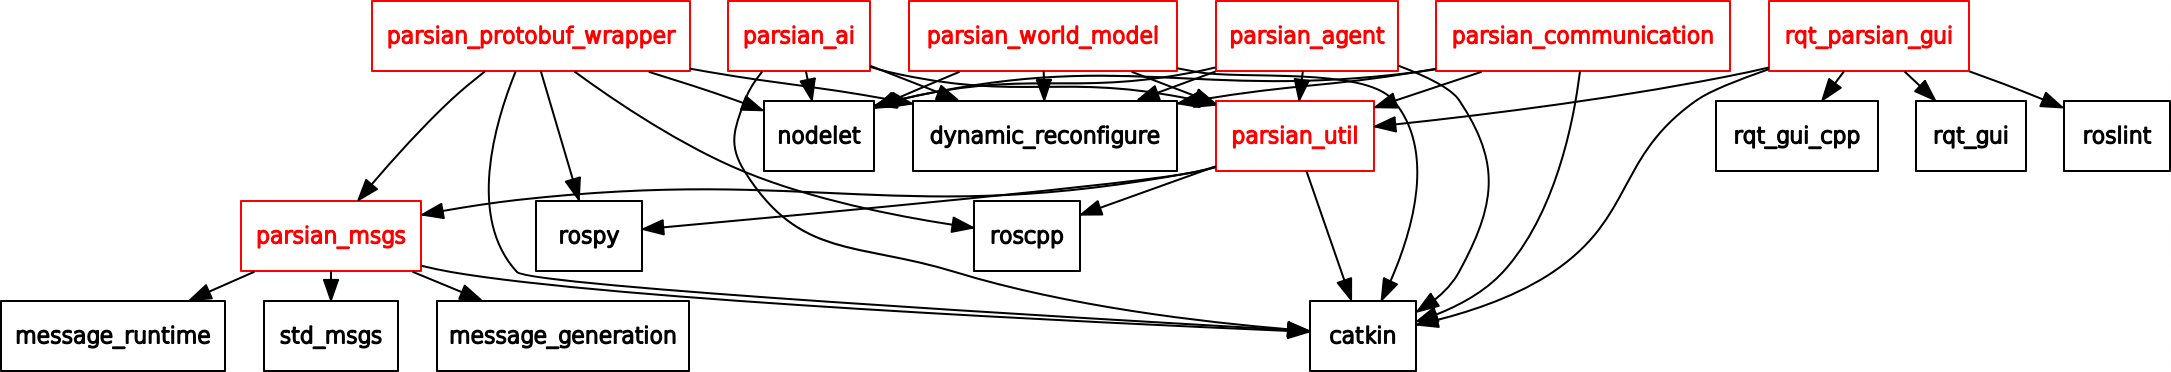
\includegraphics[width=\textwidth]{img/ai2}
\caption{Parsian packages and first-level dependencies graph}
\label{fig:AI2}
\end{figure}

\subsubsection{Node.}
\label{subsubsec:Node}
Each package has a number of nodes inside, which are actually executable files. Graph of nodes that run a game with one agent and AI is illustrated in Fig. \ref{fig:AI3}.
Nodes can be implemented with different languages and environments. They are executed separately, so when one node freezes or crashes, other ones still execute without any problem.
\ref{fig:AI2}:

\begin{figure}
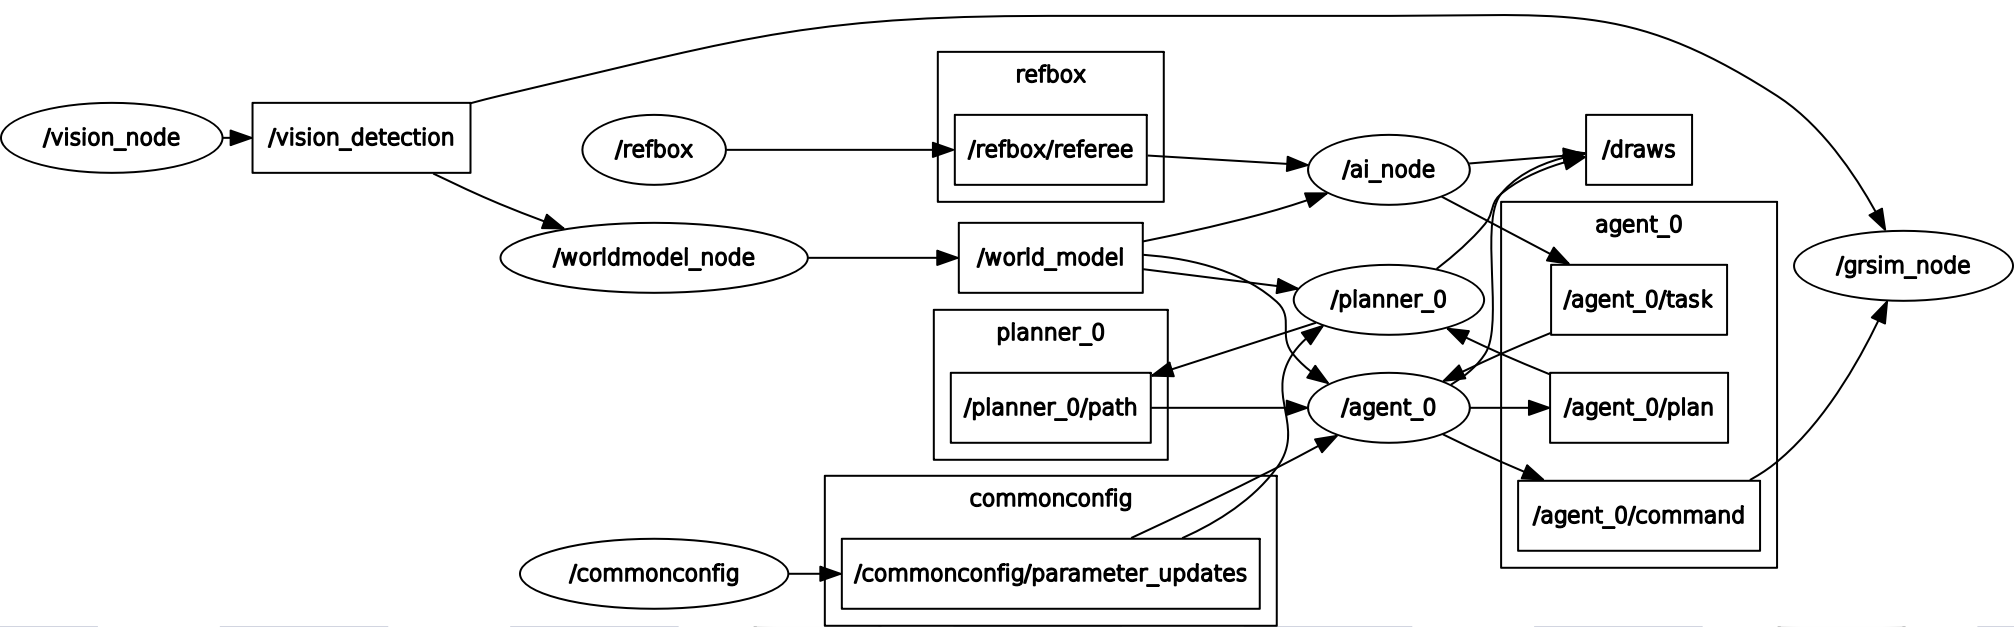
\includegraphics[width=\textwidth]{img/ai3}
\caption{Nodes and Topics graph for one agent with AI}
\label{fig:AI3}
\end{figure}

\subsubsection{Message.}
	  The most important part of designing a distributed service, is defining the messages that are going to be passed between nodes. This project tries to use pre-defined ROS messages as much as possible, to make it easier for integration with currently implemented services and nodes. You can find Parsian messages, in its repository: \url{https://github.com/ParsianRoboticLab/parsian_msgs}

\subsection{Implementation}
\label{subsec:Implementation}
\subsubsection{Latency and Delay.}
\label{subsubsec:LAtencyAndDelay}
ROS framework has lacked real-time node and services, mostly because of the latencies that serializing and parsing of messages cause, although it is not always necessary to have low latency, in GUIs for instance. The solution to resolve this latency is using \textit{nodelet} for c++ nodes. (Table \ref{tab:l})
\begin{table}
\caption{Latency of Message Passing}\label{tab:l}
\begin{center}
\begin{tabular}{l|ccc|cccl}
\hline
\multicolumn{1}{l|}{\rule{0pt}{20pt}Measured parameter} & \multicolumn{3}{c|}{Nodelet} & \multicolumn{3}{c}{Node}\\[2pt]
& Mean & Min & Max & Mean & Min & Max \\[3pt]
\hline
world model (heavy message) & 0.039 ms &  0.073 ms & 0.51 ms &
0.134 ms & 0.885 ms & 3.398 ms  \\[3pt]
robot command (light message) & 0.024 ms &  0.058 ms & 0.42 ms 
& 0.064 ms & 0.565 ms & 3.232 ms\\[3pt]
All message (critical path*) & 0.494 ms  & 0.163 ms & 3.220 ms & 3.4634 ms & 0.490 ms  & 32.763 ms\\[2pt]

\hline
\end{tabular}
\end{center}
\end{table}

\subsubsection{Nodelet.}
\label{subsubsec:Nodelet}

Nodelets are a type of ROS nodes, designed to run multiple nodes in a single process, with each node running as a plugin with the help of \textit{pluginlib}.
\newline At the very first glance, nodelets are exactly like nodes, but there is a fundamental difference between them; nodes are executable and can be run separately, whereas nodelets are not executable; they are just a software component that are loaded as plugins on a special node, called \textit{nodelet manager}.
\newline Regular nodes use TCP protocol (although if nodes run on one single PC, the shared-memory protocol supersedes TCP protocol). This works fine in most cases, but if you have multiple processes that need to use messages that contain large amounts of data exchange, then packaging the message, sending and unpacking it can take too much time. If the two processes are on the same computer, it is quicker to just send a pointer to that data rather than sending the data itself via shared-memory.
\newline Nodelet only works for processes on the same computer, since a pointer for one computer doesn't make sense for another ones. Nodes, on the other hand, can work on connected computers over network, since you're sending the actual data. To fix this problem a node is written for each nodelet as its nodelet manager. So the nodes have become entirely independent and it’s possible to continue work over networked computers.
\subsubsection{Multi-agent.}
\label{subsubsec:MUltiagent}
Since execution of robot’s skill is independent to each other, they can be run in parallel; so there is a separate node for each robot, in which the robot's operations and tasks is handled. \textit{Agent-Node} generates its own robot's commands and send them via ROS message.

\subsubsection{Path Planner Node.}
\label{subsubsec:PathPlannerNode}
	Path planner node is separated from main agent nodes, and run beside them. Advantage of this separation is:
    \begin{enumerate}
    \item Path planning is run in a different process, parallel with agent nodes, so there would be more \textit{CPU Utilization}.
    \item If a task takes too much time to complete, it won’t effect main control task, and command for robots will publish at a same frequency.
    \item Development and debug of planner can be easily done by sending and receiving messages.
    \end{enumerate}

\subsubsection{Strategy Server.}
\label{subsubsec:StrategyServer}
There are strategy files for static plays in free-kicks\cite{p:15}. Based on situation, a strategy should be chosen to run. Loading strategies, finding the best one that matches the game situation, and also analyzing the result of the selected strategy execution, are gathered into a node named \textit{strategy-server}. The routine of strategy selection service:
\begin{enumerate}
	\item  In free kicks, AI node sends a request to \textit{strategy-server node} that includes game state and a list of players.
	\item  \textit{strategy-server node} first collects some strategies that can be executed considering the data received from AI node.
	\item Chooses the best one, based on its history, and sends the strategy to AI node as a response.
    \item Evaluating the executed strategy is implemented in AI node and the result is sent back to strategy-server to be analyzed. These data is recorded and will influence the next strategy selection.
\end{enumerate}

\subsubsection{GUI and rqt}

\textit{rqt} is a Qt-based framework for GUI development in ROS. rqt makes it easier to manage the various windows on the screen at the same time. A GUI is developed in a separated node for each widget. All GUI processes run separately and use message passing to communicate with other nodes. (Fig. \ref{fig:GUI1})
\begin{figure}
\centering
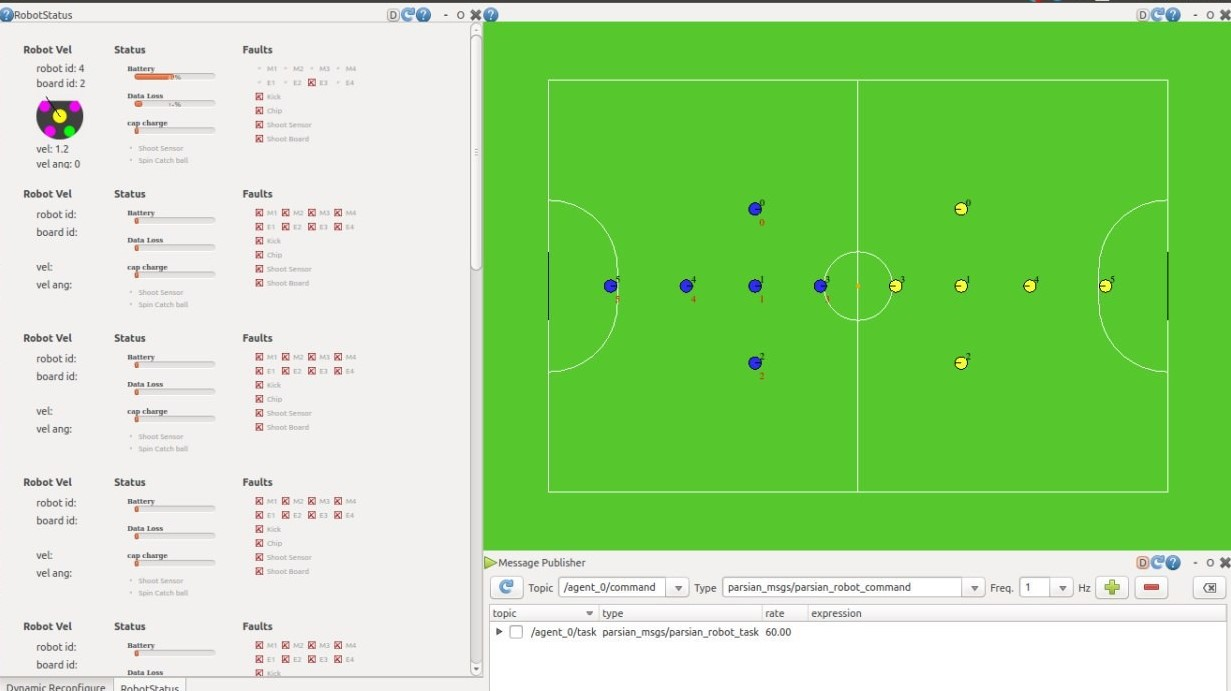
\includegraphics[width=0.60\textwidth]{img/gui1}
\centering
\caption{Robot status and monitor widget in rqt}
\label{fig:GUI1}
\end{figure}


%
\newpage

\section{Conclusion}
As Robocup SSL rules has changed recently, AI and behavior will be updated to be compatible with new rules. 
\newline
Also major work on passing and receiving in dynamic plays, started in 2016\cite{p:16}, will be used in a real game, since time calculation with new \textit{Kalman Filter} and \textit{motion profiler} is now accurate enough to execute passing.
\newline
Last year, auto-profiler and log analyzer were proven to be very useful. In Iran Open and Robocup 2017\cite{p:17}, auto-profiling and log analyzing, greatly reduced the amount of team setup time, which allowed the team to focus more on strategy planning. Although the main software that was built in 2008, and improved each year, has given successful competition result for the last years (the result summarized in Table \ref{tab:achive}, changing old monolithic software architecture to distributed in this year, was another enormous work that makes a great advantage to develop, test and debug system. Also the huge number of open-source project helped not to reinvent the wheel.
\newline
This year, Parsian hardware's changes aim to stabilize robots with detecting and monitoring their faults. Next steps are online configuration of robot's low-level parameters, and then auto-calibrating the controller's parameters along the game.
\newline
In control part, motion controller is improved greatly by improving \textit{Kalman Filter}, \textit{open-loop calibration} and \textit{motion profiler}; most important outcome is accurate timing for robot's movement.


\begin{table}
\caption{Parsian Achievements}\label{tab:achive}
\begin{center}
\begin{tabular}{r@{\quad}rl}
\hline
\multicolumn{1}{c}{\rule{0pt}{12pt}Year} & \multicolumn{2}{c}{Result}\\[2pt]
\hline\rule{0pt}{12pt}
RoboCup 2014  &     Round Robin& \\
RoboCup 2015  &     Lucky Loser& \\
RoboCup 2016  &     Lucky Loser& \\
RoboCup 2017  &     4th Place  & \\[2pt]
\hline
\end{tabular}
\end{center}
\end{table}

\newpage

\begin{thebibliography}{5}
%
\bibitem {p:17}
Rahimi, M., Shirazi, M., Arfaee, M., Najaf Gholian, M., Zamani, A., Hosseini, H., Hashemi, F., Moradi, N., Ahsani, A., Jafari, M., Zahedi, A., Abdoullahi, P., Zolanvari, A., Khosravi, M.:
Parsian 2017 Extended Team Description Paper for RoboCup. (2017)

\bibitem {p:16}
Rahimi, M., Shirazi, M., Dajkhosh, P., Zolanvari, A., Arfaee, M., Kazemi H., Abbasi, A., Saeidi, A., Khosravi, M.:
Parsian 2016 Extended Team Description Paper for RoboCup. (2016)

\bibitem {p:15}
Zolanvari, A., Shirazi, M., Dajkhosh, P., Naderi, M., Arfaee, M., Behbooei, M., Kazemi H., Tazimi, E., Rahimi, M., Saeidi, A.,:
Parsian 2015 Extended Team Description Paper for RoboCup. (2015)

\end{thebibliography}

\end{document}
